% THIS IS SIGPROC-SP.TEX - VERSION 3.1
% WORKS WITH V3.2SP OF ACM_PROC_ARTICLE-SP.CLS
% APRIL 2009
%
% It is an example file showing how to use the 'acm_proc_article-sp.cls' V3.2SP
% LaTeX2e document class file for Conference Proceedings submissions.
% ----------------------------------------------------------------------------------------------------------------
% This .tex file (and associated .cls V3.2SP) *DOES NOT* produce:
%       1) The Permission Statement
%       2) The Conference (location) Info information
%       3) The Copyright Line with ACM data
%       4) Page numbering
% ---------------------------------------------------------------------------------------------------------------
% It is an example which *does* use the .bib file (from which the .bbl file
% is produced).
% REMEMBER HOWEVER: After having produced the .bbl file,
% and prior to final submission,
% you need to 'insert'  your .bbl file into your source .tex file so as to provide
% ONE 'self-contained' source file.
%
% Questions regarding SIGS should be sent to
% Adrienne Griscti ---> griscti@acm.org
%
% Questions/suggestions regarding the guidelines, .tex and .cls files, etc. to
% Gerald Murray ---> murray@hq.acm.org
%
% For tracking purposes - this is V3.1SP - APRIL 2009

\documentclass{sig-alternate-ipsn13}

%-----------------------------------------
% need for camera-ready
\pagestyle{empty}

%----------------------------------------

\begin{document}

\title{
Zero-Copy I/O Processing for Real-Time GPU Applications
}
%
% You need the command \numberofauthors to handle the 'placement
% and alignment' of the authors beneath the title.
%
% For aesthetic reasons, we recommend 'three authors at a time'
% i.e. three 'name/affiliation blocks' be placed beneath the title.
%
% NOTE: You are NOT restricted in how many 'rows' of
% "name/affiliations" may appear. We just ask that you restrict
% the number of 'columns' to three.
%
% Because of the available 'opening page real-estate'
% we ask you to refrain from putting more than six authors
% (two rows with three columns) beneath the article title.
% More than six makes the first-page appear very cluttered indeed.
%
% Use the \alignauthor commands to handle the names
% and affiliations for an 'aesthetic maximum' of six authors.
% Add names, affiliations, addresses for
% the seventh etc. author(s) as the argument for the
% \additionalauthors command.
% These 'additional authors' will be output/set for you
% without further effort on your part as the last section in
% the body of your article BEFORE References or any Appendices.

\numberofauthors{2} %  in this sample file, there are a *total*
% of EIGHT authors. SIX appear on the 'first-page' (for formatting
% reasons) and the remaining two appear in the \additionalauthors section.
%
\author{
% You can go ahead and credit any number of authors here,
% e.g. one 'row of three' or two rows (consisting of one row of three
% and a second row of one, two or three).
%
% The command \alignauthor (no curly braces needed) should
% precede each author name, affiliation/snail-mail address and
% e-mail address. Additionally, tag each line of
% affiliation/address with \affaddr, and tag the
% e-mail address with \email.
%
\alignauthor Shinpei Kato\\
       \affaddr{Dept. Information Engineering}\\
       \affaddr{Nagoya University}
\and
\alignauthor Nikolaus Rath\\
       \affaddr{Dept. Applied Physics and Applied Mathematics}\\
       \affaddr{Columbia University}
\and
\alignauthor Jason Aumiller and Scott Brandt\\
       \affaddr{Dept. Computer Science}\\
       \affaddr{University of California, Santa Cruz}
}
% There's nothing stopping you putting the seventh, eighth, etc.
% author on the opening page (as the 'third row') but we ask,
% for aesthetic reasons that you place these 'additional authors'
% in the \additional authors block, viz.
%\additionalauthors{Additional authors: John Smith (The Th{\o}rv{\"a}ld Group,
%email: {\texttt{jsmith@affiliation.org}}) and Julius P.~Kumquat
%(The Kumquat Consortium, email: {\texttt{jpkumquat@consortium.net}}).}
%\date{30 July 1999}
% Just remember to make sure that the TOTAL number of authors
% is the number that will appear on the first page PLUS the
% number that will appear in the \additionalauthors section.

\maketitle

%-----------------------------------------
% need for camera-ready
\thispagestyle{empty}

\begin{abstract}
 Cyber-physical systems (CPS) often control complex physical
 phenomenon. 
 The computational workload of control algorithms, hence, is becoming a
 core challenge of CPS due to their real-time constraints.
 By nature, control algorithms of CPS exhibit a high degree of data
 parallelism, which can be offloaded to parallel compute devices,
 such as graphics processing units (GPUs).
 Yet another problem is introduced by the communication between the host
 processor and the compute device.
 As a matter of fact, plasma control requires an order of a few
 microseconds for the sampling period, while today's systems may take
 several ten microseconds to copy data between the host and the device
 memory at scale of the required data size.
 In this paper, we present a zero-copy I/O processing scheme that
 enables sensor and actuator devices to directly transfer data to and
 from compute devices without using the host processor.
 The basic idea behind this scheme is to map the I/O address space onto
 the device memory, removing data-copy operations upon the host memory.
 The experimental results from the real-world plasma control
 system demonstrate that a sampling period of plasma control can be
 reduced by 33\% under the zero-copy I/O scheme.
 The microbenchmarking results also show that GPU-accelerated matrix
 computations can be completed in 34\% less time than current methods,
 while effective data throughput is at least as good as the current best
 performers.
\end{abstract}

\keywords{GPGPU, Zero-Copy I/O, Plasma Fusion}

\section{Introduction}
\label{sec:introduction}

Cyber-physical systems (CPS) are next generations of networked and
embedded systems, tightly coupled with computation and physical
elements to control real-world phenomenon.
Control algorithms of CPS, therefore, are becoming more and more
complex, which makes CPS distinguished from traditional safety-critical
systems.
In CPS applications, ``real-fast'' is often as important as ``real-time'',
while safety-critical systems are likely to have only the real-time
constraint. 
Such a double-edge real-time and real-fast requirement of CPS, however,
has imposed a core challenge on systems technology.
In this paper, we tackle this problem with a specific example of plasma
control.

\begin{figure}[tb]
 \centering
 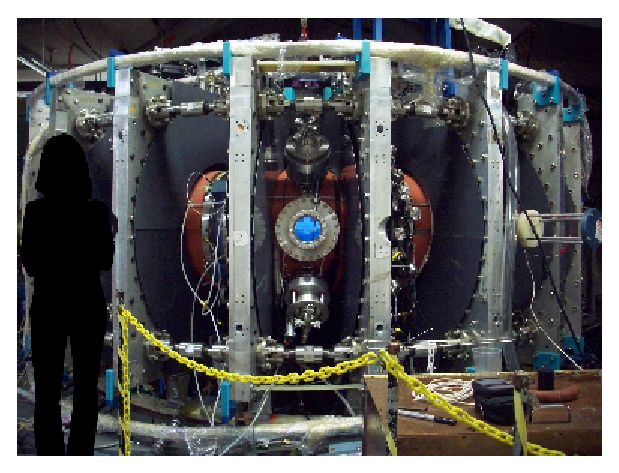
\includegraphics[width=0.8\hsize]{eps/tokamak.eps}
 \caption{The HBT-EP ``Tokamak'' at Columbia University.}
 \label{fig:tokamak}
\end{figure}

Plasma control for fusion is an applications of energy CPS, where
complex algorithms must be computed at a very high rate.
Figure~\ref{fig:tokamak} shows the HBT-EP Tokamak at Columbia
University~\cite{Maurer_PPCF11,Rath_FED12} that magnetically controls
the 3-D perturbed equilibrium state of the plasma~\cite{Boozer_PP99}.
It is required to process 96 inputs and 64 outputs of 16-bit data at a
sampling rate of a few microseconds.
An initial attempt of the Columbia team employed fast CPUs or FPGAs, but
even the simplified algorithm failed to run within 20$\mu$s.
An alternative approach was to parallelize the algorithm using the
graphics processing unit (GPU) and CUDA~\cite{CUDA} -- the most
successful massively parallel computing technology.
However, the current system for GPU computing is not designed to
integrate sensor and actuator devices with the GPU.
This is attributed to the fact that the current software stack
of GPU computing is independent of I/O device drivers.
Since it might take tens of microseconds to transfer hundreds-of-bytes
data between the CPU and the GPU, it is not affordable for the current
software stack to apply the GPU for plasma control in real-time.
This is a signficant problem not only for plasma control but also for
any applications of CPS that are augmented with compute devices.

In order to utilize the GPU for applications of CPS, the system is
required to support a method of bypassing data transfer between the GPU
and the CPU, instead connecting the GPU and I/O devices directly.
To the best of our knowledge, however, there is currently no generic
systems support for such a direct data transfer machanism except for
specialized commercial products for the InfiniBand
network~\cite{GPUDirect}.
As a way of eliminating the data transfer cost between the CPU and the
GPU, the current programming framework often supports host memory
allocation, which enables the GPU to access data on the host memory;
however, it is unclear if this scheme is best suited for low-latency GPU
computing, because the data access to the host memory from the GPU is
expensive.
Given that GPUs are increasingly deployed in the domain of
CPS~\cite{Hirabayashi_REACTION12, Mangharam11, McNaughton_ICRA11,
Michel_IROS07}, 
and basic real-time resource management techniques for the GPU started to be
disclosed \cite{Elliott_RTS12, Elliott_ECRTS12, Kato_RTAS11,
Kato_RTSS11, Kato_ATC11, Kato_ATC12, Liu_PACT12}, it is time to look
into a tight integration of I/O processing and GPU computing.

\textbf{Contribution:}
In this paper, we present a zero-copy I/O processing scheme for GPU
computing.
This scheme enables I/O devices to directly transfer a limited size of
data to and from the GPU, by coordinating their device drivers. 
We also investigate a possibility of the exisiting schemes to support
low-latency GPU computing, and identify an advantage of our new scheme.
To do so, we provide a case study using the Columbia University's
Tokamak plasma control system that demonstrates an effect of our
new scheme on a sampling period of plasma control.
Furthermore, we provide microbenchmarking results to evaluate more
generic properties of the I/O processing schemes
By clarifying these capabilities, we aim to not only improve the overall
performance but also broaden the scope of CPS that can benefit from the
state-of-the-art GPU computing technology.

\textbf{Organization:}
The rest of this paper is organized as follows.
Section~\ref{sec:system_model} describes the system model and
assumptions behind this paper.
Section~\ref{sec:io_processing} presents our zero-copy I/O processing
scheme, and differentiates it from the exisiting schemes.

\bibliographystyle{abbrv}
\bibliography{references}

\end{document}
